% 隔離テスト用ドライバ: 14-17 のみを単独ビルド（共有 main.tex には影響しない）
% 担当: スライド 14-17。main.* には一切触れない。
\documentclass[11pt,aspectratio=43,dvipsnames]{beamer}
\usepackage{luatexja}
\usepackage[match]{luatexja-fontspec}
\setmainjfont{HaranoAjiGothic}
\setsansjfont{HaranoAjiGothic}
\renewcommand{\kanjifamilydefault}{\gtdefault}
\usepackage{amsmath, amssymb}
\usepackage[version=4]{mhchem}
\usepackage{booktabs}
\usepackage{multirow}
\usepackage{colortbl}
\usepackage{graphicx}
\graphicspath{{figures/}}
\usepackage{pgfplots}
\pgfplotsset{compat=1.18}
% =====================================================================
%  seminar テーマ定義（既存 Marp デザインの Beamer 再現）
%  ・濃青の恒常ヘッダーバー（セクション名＋ページ番号）
%  ・専用表紙（アクセントライン＋グラデ背景）
%  ・本文は白地・濃青見出し
%  main.tex から \input する（パッケージではなく生プリアンブル）
% =====================================================================

% ---- ベース：装飾の少ないテーマから組む -----------------------------
\usetheme{default}
\usefonttheme{professionalfonts}
\setbeamertemplate{navigation symbols}{}   % ナビゲーション記号を消す

% ---- TikZ（ヘッダー・表紙・矢印などで使用）-------------------------
\usepackage{tikz}
\usetikzlibrary{arrows.meta, positioning, calc, shapes.geometric, fit, patterns}

% ---- 配色（ルール準拠）---------------------------------------------
\definecolor{HeaderBlue}{HTML}{0f5a7a}   % ヘッダー・見出しの濃青
\definecolor{DateGray}{HTML}{334b5e}     % 表紙の日付グレー
\definecolor{TitleBG}{HTML}{edf5fb}      % 表紙グラデの薄青

% コンテンツ用パレット（図・ハイライト・矢印で共通利用）
\definecolor{ArrowBlue}{HTML}{1F6FC4}    % 矢印・強調の青
\definecolor{HiPink}{HTML}{F4B6BE}       % ハイライト見出し（暖色）
\definecolor{HiBlue}{HTML}{C7DCEF}       % ハイライト見出し（寒色）
\definecolor{IpaBlue}{HTML}{1F5FC4}      % グラフ系列1（青）
\definecolor{DipeOrange}{HTML}{E8821E}   % グラフ系列2（橙）
\definecolor{SpRed}{HTML}{C0392B}        % 反応式：プロピレン強調の赤
\definecolor{SpBlue}{HTML}{1F6FC4}       % 反応式：エテン・エタン・CH0.5 の青

% 帯（ヘッダーバー）のパート別配色（寒色グラデ）。本文枠線は HeaderBlue のまま。
%  1-4 導入・全体像／5-9 反応・反応器／10-13 分離／14-17 最適化・経済・結言
\definecolor{barA}{HTML}{0F5A7A}   % 1-4  青緑
\definecolor{barB}{HTML}{1D6E6E}   % 5-9  シアン寄り
\definecolor{barC}{HTML}{2E4C8A}   % 10-13 青
\definecolor{barD}{HTML}{4A3C84}   % 14-17 紫

\setbeamercolor{normal text}{fg=black, bg=white}
\setbeamercolor{frametitle}{fg=HeaderBlue, bg=white}
\setbeamercolor{itemize item}{fg=HeaderBlue}
\setbeamercolor{itemize subitem}{fg=HeaderBlue}
\setbeamercolor{block title}{fg=white, bg=HeaderBlue}
\setbeamercolor{block body}{fg=black, bg=TitleBG}
\setbeamercolor{alerted text}{fg=HeaderBlue}

% ---- フォントサイズ（Marp px をおおよそ pt に対応）------------------
\setbeamerfont{frametitle}{size=\large, series=\bfseries}   % スライド見出し ~44px

% ---- 恒常ヘッダーバー（headline）-----------------------------------
%  左：セクション名（無ければロゴ枠）／右：ページ番号
\newcommand{\HeaderLogo}{}   % ロゴを入れるなら \renewcommand で画像指定
% 本線の総枚数（分母）。appendix に入ると分子がこれを超え、本線/付録を見分けられる。
\newcommand{\MainTotal}{17}
% パート別に帯色を選ぶ：1-4=barA／5-9=barB／10-13=barC／14-17=barD。
% スライド4の独自帯（CC・GCC）など headline を上書きする箇所でも呼べるよう独立コマンド化。
% 併せて本文アクセント色 HeaderBlue 自体をそのパート色へ再定義し、各スライドの
% 図・枠線・矢印・ボックス（HeaderBlue 参照）をパート色に連動させる（\colorlet は大域的）。
% headline はフレーム本文より前に組まれるため、ここでの再定義が本文に効く。
\newcommand{\SetBarColor}{%
  \ifnum\insertframenumber<5\setbeamercolor{headerbar}{fg=white, bg=barA}\colorlet{HeaderBlue}{barA}%
  \else\ifnum\insertframenumber<10\setbeamercolor{headerbar}{fg=white, bg=barB}\colorlet{HeaderBlue}{barB}%
  \else\ifnum\insertframenumber<14\setbeamercolor{headerbar}{fg=white, bg=barC}\colorlet{HeaderBlue}{barC}%
  \else\setbeamercolor{headerbar}{fg=white, bg=barD}\colorlet{HeaderBlue}{barD}%
  \fi\fi\fi}
\setbeamertemplate{headline}{%
  \ifnum\insertframenumber>0\relax
    \SetBarColor
    \begin{beamercolorbox}[wd=\paperwidth, ht=4.5ex, dp=1.8ex,
                           leftskip=1.2em, rightskip=1.2em]{headerbar}%
      \color{white}\bfseries\large
      \insertsectionhead%
      \hfill
      \insertframenumber/\MainTotal%
    \end{beamercolorbox}%
  \fi
}
\setbeamercolor{headerbar}{fg=white, bg=barA}
\setbeamertemplate{footline}{}             % フッターは使わない
\setbeamersize{text margin left=3mm, text margin right=3mm}  % 本文を横幅ぎりぎりまで

% 【必須ルール】帯と本文の間の余白を詰める（全スライド共通）。
%  beamer 既定の天井スキップで本文が帯から離れるのを、headline 直後の負スキップで打ち消す。
%  情報量最優先：無駄な上余白は作らない。各スライドは [t] 推奨。
\addtobeamertemplate{headline}{}{\vskip-2.6ex}

% frametitle はバーの直下に置く（左寄せ・濃青・太字）
\setbeamertemplate{frametitle}{%
  \vskip0.6ex
  \hspace{0.6em}\usebeamerfont{frametitle}\usebeamercolor[fg]{frametitle}\insertframetitle\par
  \vskip0.2ex
}

% ---- 箇条書きをシンプルに ------------------------------------------
\setbeamertemplate{itemize item}{\textbullet}
\setbeamertemplate{itemize subitem}{--}

% =====================================================================
%  再利用ヘルパー（どのスライドでも使える共通部品）
% =====================================================================
% 青い矢印 →（行中に置ける。結論や対応関係の明示に）
\newcommand{\bluearrow}{\tikz[baseline=-0.5ex]\draw[ArrowBlue, line width=1pt,
  -{Stealth[length=2.2mm]}] (0,0)--(0.55,0);}

% ハイライト見出し  \hilite{色}{テキスト}  例: \hilite{HiPink}{IPA選択率の温度依存性}
\newcommand{\hilite}[2]{\colorbox{#1}{\bfseries\normalsize #2}}

% パラメータ表  \paramtable{ 項目 & 値 \\ ... }  （左:項目 右:値、単位は数式推奨）
\newcommand{\paramtable}[1]{%
  {\footnotesize\renewcommand{\arraystretch}{1.15}%
   \begin{tabular}{@{\hspace{1em}}ll@{}}#1\end{tabular}}}

% =====================================================================
%  専用表紙コマンド  \seminartitlepage
%  ルール準拠：アクセントライン(120x8px相当) + 160度グラデ背景
%               h1 60px / h2 34px濃青 / 著者27px / 日付22pxグレー
%  使い方: \title{} \subtitle{} \author{} \date{} を設定後に呼ぶ
% =====================================================================
\newcommand{\seminartitlepage}{%
  \begin{frame}[plain]
    \begin{tikzpicture}[remember picture, overlay]
      % 背景グラデ（左上 薄青 → 右下 白、斜め）
      \shade[top color=TitleBG, bottom color=white, shading angle=20]
        (current page.south west) rectangle (current page.north east);
      % アクセントライン（上から少し下げて左に）
      \fill[HeaderBlue]
        ([xshift=9mm, yshift=-12mm]current page.north west)
        rectangle ++(16mm, 1.1mm);
      % テキストブロック（左寄せ・縦中央付近）
      \node[anchor=center, text width=0.86\paperwidth, align=center]
            at (current page.center) {%
        {\fontsize{22pt}{28pt}\selectfont\bfseries\color{black}\inserttitle\par}
        \vspace{0.3em}
        {\fontsize{16pt}{20pt}\selectfont\bfseries\color{HeaderBlue}\insertsubtitle\par}
        \vspace{1.0em}
        {\fontsize{13pt}{17pt}\selectfont\color{black}\insertauthor\par}
        \vspace{0.4em}
        {\fontsize{11pt}{14pt}\selectfont\color{DateGray}\insertdate\par}
      };
    \end{tikzpicture}
  \end{frame}
}

\setlength{\overfullrule}{6pt}
\begin{document}
\setcounter{framenumber}{13}
\section{全体最適化}% =====================================================================
%  14  全体最適化 — 左=手法／評価関数(TAC・CAPEX・OPEX の定義と分類)／制約、
%   右=設計変数22の探索範囲＋最適化で決定した値(赤)。F_freshは従属変数のため非掲載。
%  source_memo: 評価関数・CAPEX/OPEX 定義=03_economic_indicators.tex（TAC=CAPEX/n+OPEX, n=8、
%   OPEX=0.180 C_TM+2.73 C_OL+1.23(C_UT+C_WT+C_RM)）、探索範囲=Z:\pdh_simulator\main.py SEARCH_SPACE、
%   決定値=02_process_overview.tex Table 2.3 / best.json trial #201（スライド3と一致）、
%   制約=Z:\pdh_simulator\flowsheet\specs.py＋units\reactors\catofin.py。
%  方針：帯と本文を重ねない（上 vspace は小さな正）。余白を先に使い、足りない分だけ縮小。
%        評価関数を主役に TAC/CAPEX/OPEX の定義・分類を詳述。決定値は赤＝最適化の出力。丸括弧禁止。
% =====================================================================
\definecolor{SpGreen}{HTML}{1FB24D}   % 製品目標スペック強調用の明るい緑
\begin{frame}[t]

  \vspace*{0.2ex}
  \begin{columns}[T,onlytextwidth]
    % ===== 左：最適化手法・評価関数(TAC/CAPEX/OPEX 詳述)・制約条件 ====
    \begin{column}{0.53\textwidth}
      \fbox{\scriptsize 最適化手法}\;{\footnotesize\bfseries ベイズ最適化(TPE)}\par

      \vspace{0.34em}
      \fbox{\scriptsize 評価関数}\;{\footnotesize 年間総費用 {\color{SpRed}\bfseries TAC} を最小化}\par
      \vspace{0.2em}
      {\normalsize\boldmath$ {\color{SpRed}\mathrm{TAC}}=\mathrm{CAPEX}/n+\mathrm{OPEX} $\unboldmath}\par

      \vspace{0.46em}
      {\raggedright
       {\footnotesize\bfseries CAPEX}\par
       {\scriptsize\linespread{1.05}\selectfont 資本的支出　建設の初期投資\par
        \hspace{0.9em}直接費：機器費・据付・配管・計装・土木\par
        \hspace{0.9em}間接費：設計・予備費・エンジニアリング\par}
       \vspace{0.38em}
       {\footnotesize\bfseries OPEX}\par
       {\scriptsize\linespread{1.05}\selectfont 事業運営費　年間の運転費\par
        \hspace{0.9em}変動費：原料費・用役費・廃棄物処理費\par
        \hspace{0.9em}固定費：労務費・保全費・一般経費\par
        \vspace{0.95em}
        $n$：法定耐用 $8$ 年\par}
      }

      \vspace{0.46em}
      \fbox{\scriptsize 制約条件}\par
      \vspace{0.18em}
      {\scriptsize\linespread{1.0}\selectfont
       \begin{tabular}{@{}p{0.47\linewidth}@{\hspace{0.3em}}|@{\hspace{0.3em}}p{0.50\linewidth}@{}}
         \raggedright
         {\color{SpGreen}・C3H6 純度 $\ge 99.5$ wt\%}\par
         ・H2 純度 $\ge 99.9$ mol\%\par
         {\color{SpGreen}・生産量 $\ge 400$ kt/年}\par
         ・反応器 床$\Delta P\le 5$\%\par
         ・反応器 総$\Delta P\le 10$\%\par
         ・空塔速度 $\ge 0.15$ m/s
         &
         \raggedright
         ・触媒体積 $\le 200\ \mathrm{m^3}$／基\par
         ・PSA 床圧損 $\le 0.3$ bar\par
         ・脱エタン塔頂が凝縮可\par
         ・膜供給圧 $>$ フィード圧\par
         ・リサイクル収支整合
       \end{tabular}}
    \end{column}

    \begin{column}{0.01\textwidth}\end{column}   % 中央の余白

    % ===== 右：設計変数22の探索範囲＋決定値(赤)。ユニットごとに枠を分割 ======
    \begin{column}{0.46\textwidth}
      \setlength{\fboxsep}{1.5pt}\setlength{\fboxrule}{0.8pt}%
      \fcolorbox{HeaderBlue}{white}{\makebox[\dimexpr\linewidth-2\fboxsep-2\fboxrule\relax][l]{%
        \scriptsize\renewcommand{\arraystretch}{0.82}%
        \begin{tabular}{@{}l@{\hspace{0.5em}}l@{\hspace{0.5em}}l@{\hspace{0.6em}}r@{\hspace{0.35em}}l@{}}
          入口温度     & $T_{\mathrm{in}}$  & $930$–$940$   & {\color{SpRed}$935.2$} & K \\
          サイクル時間 & $t_{\mathrm{cyc}}$ & $12$–$25$     & {\color{SpRed}$14.0$}  & min \\
          反応器内径   & $D$                & $9$–$12$      & {\color{SpRed}$10.76$} & m \\
          浅床厚       & $L_{\mathrm{bed}}$ & $0.3$–$3.0$   & {\color{SpRed}$1.58$}  & m \\
          並列基数     & $N_{\mathrm{on}}$  & $6$–$8$       & {\color{SpRed}$7$}     & --- \\
          触媒粒径     & $d_p$              & $4$–$6$       & {\color{SpRed}$5.84$}  & mm \\
        \end{tabular}}}\par\vspace{0.6pt}
      \fcolorbox{HeaderBlue}{white}{\makebox[\dimexpr\linewidth-2\fboxsep-2\fboxrule\relax][l]{%
        \scriptsize\renewcommand{\arraystretch}{0.82}%
        \begin{tabular}{@{}l@{\hspace{0.5em}}l@{\hspace{0.5em}}l@{\hspace{0.6em}}r@{\hspace{0.35em}}l@{}}
          PSA 塔径     & $D_{\mathrm{P}}$   & $2.9$–$5.0$   & {\color{SpRed}$4.49$}  & m \\
          PSA 層高     & $L_{\mathrm{P}}$   & $22$–$30$     & {\color{SpRed}$24.8$}  & m \\
          脱着基準     & $\beta$            & $0.22$–$0.40$ & {\color{SpRed}$0.254$} & --- \\
        \end{tabular}}}\par\vspace{0.6pt}
      \fcolorbox{HeaderBlue}{white}{\makebox[\dimexpr\linewidth-2\fboxsep-2\fboxrule\relax][l]{%
        \scriptsize\renewcommand{\arraystretch}{0.82}%
        \begin{tabular}{@{}l@{\hspace{0.5em}}l@{\hspace{0.5em}}l@{\hspace{0.6em}}r@{\hspace{0.35em}}l@{}}
          膜供給圧     & $P_H$              & $7.5$–$9.5$   & {\color{SpRed}$8.44$}  & bar \\
          膜面積       & $A_{\mathrm{mem}}$ & $0.5$–$3$     & {\color{SpRed}$1.28$}  & $\times10^{5}\,\mathrm{m^2}$ \\
        \end{tabular}}}\par\vspace{0.6pt}
      % 原料流量 F_fresh は最適化変数ではなく従属変数（製品スペック固定下で物質収支から決定、
      % 決定値 1494.6 kmol/h）のため本表から除外（22 変数）。
      \fcolorbox{HeaderBlue}{white}{\makebox[\dimexpr\linewidth-2\fboxsep-2\fboxrule\relax][l]{%
        \scriptsize\renewcommand{\arraystretch}{0.82}%
        \begin{tabular}{@{}l@{\hspace{0.5em}}l@{\hspace{0.5em}}l@{\hspace{0.6em}}r@{\hspace{0.35em}}l@{}}
          塔圧力       & $P_1$ & $16$–$20$    & {\color{SpRed}$19.5$} & bar \\
                       & $P_2$ & $7.7$–$8.2$  & {\color{SpRed}$7.88$} & bar \\
                       & $P_3$ & $16$–$19$    & {\color{SpRed}$16.8$} & bar \\
          塔段数       & $N_1$ & $30$–$60$    & {\color{SpRed}$36$}   & --- \\
                       & $N_2$ & $60$–$80$    & {\color{SpRed}$61$}   & --- \\
                       & $N_3$ & $115$–$160$  & {\color{SpRed}$117$}  & --- \\
          フィード段   & $N_{f1}$ & $22$–$28$ & {\color{SpRed}$28$}   & --- \\
          フィード比   & $f_2$ & $0.40$–$0.60$ & {\color{SpRed}$0.51$} & --- \\
                       & $f_3$ & $0.60$–$0.90$ & {\color{SpRed}$0.82$} & --- \\
          組成分率     & $\phi_1$ & $0.90$–$0.999$ & {\color{SpRed}$0.995$} & --- \\
          還流比       & $R_2$ & $10$–$15$    & {\color{SpRed}$11.8$} & --- \\
        \end{tabular}}}\par
      \vspace{1pt}
      {\tiny {\color{SpRed}\bfseries 赤：決定値}・$1$脱ブタン $2$脱エタン $3$C3塔}
    \end{column}
  \end{columns}

\end{frame}

\section{最適化変数の選定}% =====================================================================
%  15  最適化変数の選定 — 「変数の最適値は互いに依存＝部分最適化できない」を
%   工程をまたぐ4つの変数ペアの TAC 等高線(全点フローシート HYSYS, trial#201 背景)で示す。
%   どのペアでも最小 TAC の谷が斜め＝2変数の最適値が互いに依存 → 全 23 変数を同時最適化。
%  source_memo: figures/make_interaction_panels.py(+ run_interaction_grid.py /
%   run_interaction_xsub.py が p1..p4 を全フローシート評価)。★＝採用設計。
% =====================================================================
\begin{frame}[t]

  \vspace*{2.0ex}
  {\bfseries\normalsize 最適値が相互依存　$\to$　全 23 変数を同時最適化}\par

  \vspace{0.6ex}
  \centering
  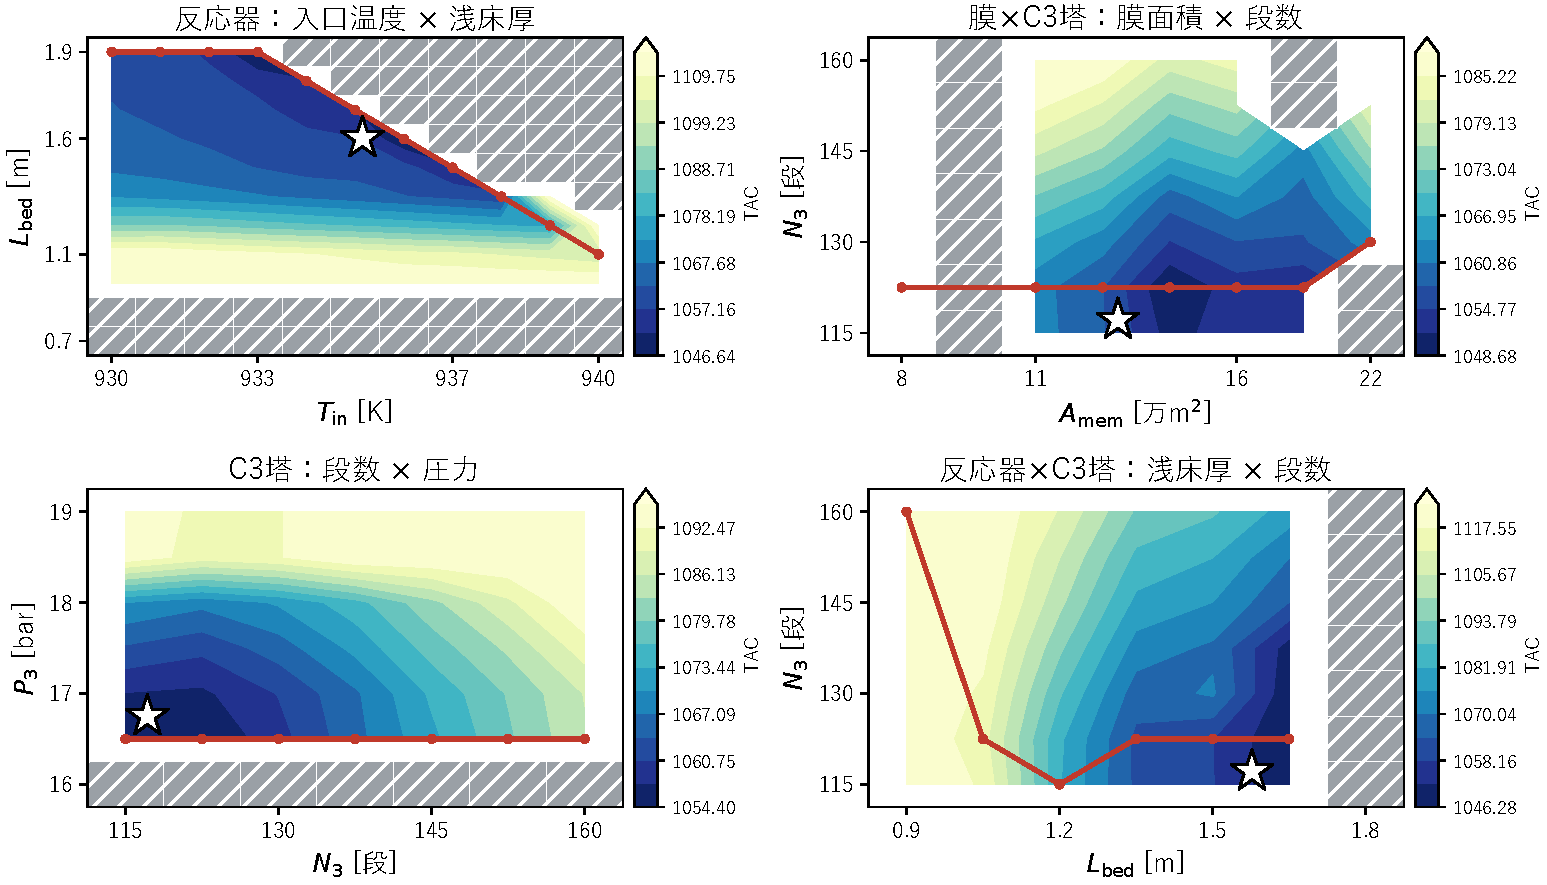
\includegraphics[width=0.95\linewidth]{fig_interaction_panels}\par
  \vspace{0.2ex}
  {\scriptsize 各ペアの TAC 等高線（☆：採用設計・灰：制約違反・{\color{SpRed}赤線}：各列で TAC 最小の点＝谷底）}\par
  \vspace{0.25em}
  {\scriptsize どのユニットでも 2 変数の最適な組合せは互いに依存し独立に決められない}

\end{frame}

\section{経済性}% =====================================================================
%  16  経済分析 — 費用/収益・OPEX/CAPEX 内訳（上段）と世界 PDH 立地（下段）
%  source_memo: 10_optimization.tex §経済性・12_analysis_discussion.tex §採算性/立地。
%   図 figures/make_econ_breakdown_slide.py（棒＋OPEX/CAPEX ドーナツ, OPEX は HI 後）と
%      figures/make_econ_map_slide.py（米州｜欧中亜の 2 パネル）。
%   いずれも graph/make_charts.py・make_map.py と同一データをスライド用に変換。
%  方針：見出し文は置かず図で語らせる。図は \paperwidth で左右フルブリード、
%   上は帯直下・下は最下部まで使い、余白を最小化する。丸括弧禁止。
% =====================================================================
\begin{frame}[t]

  \vspace*{6mm}   % 帯とタイトルの重なり回避：内容を明示的に下げる（[t] では \fill が効かないため）
  \centering
  \makebox[\linewidth]{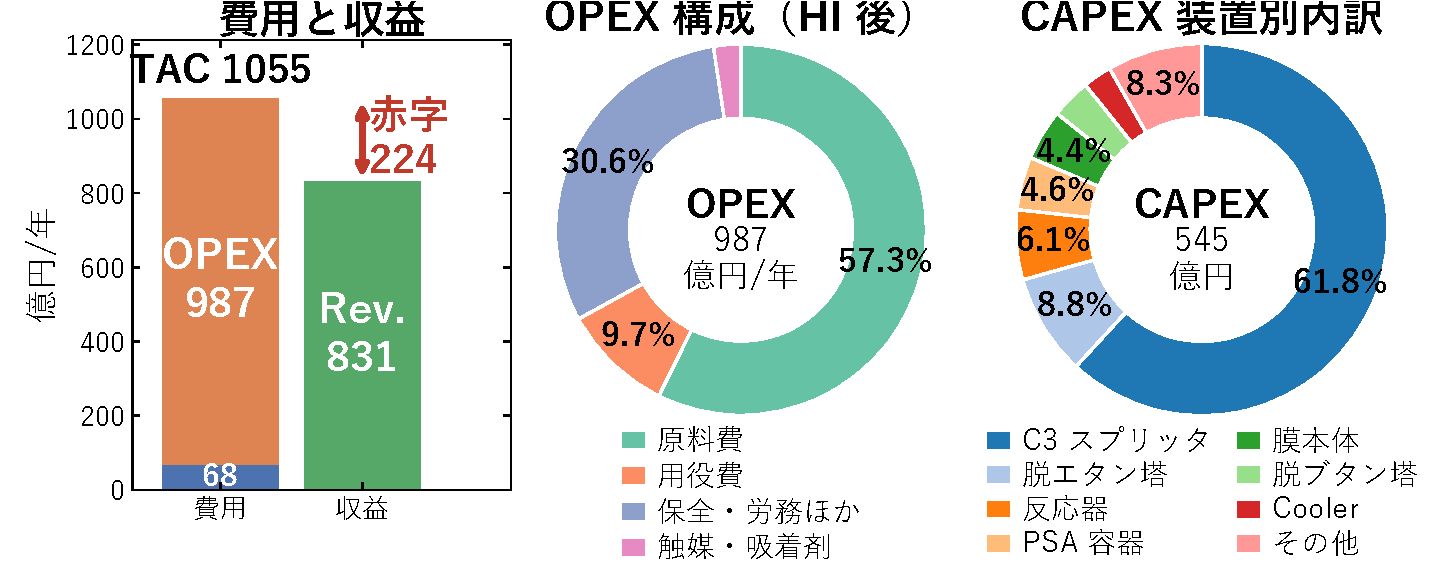
\includegraphics[width=\paperwidth]{econ_breakdown_slide}}\par

  \vspace{0.1em}
  \makebox[\linewidth]{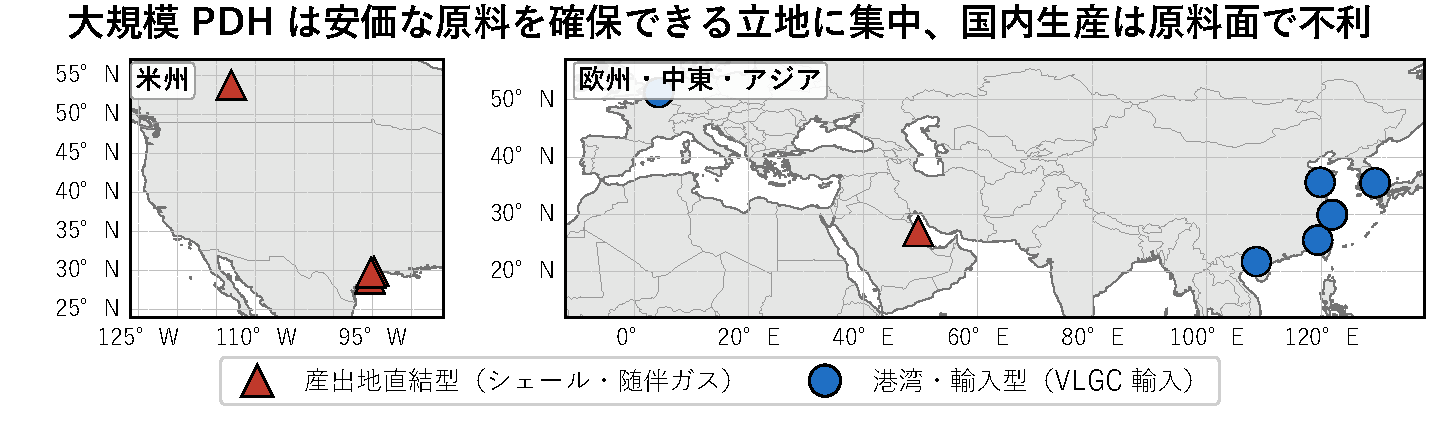
\includegraphics[width=\paperwidth]{econ_map_slide}}

\end{frame}

\section{結言}% =====================================================================
%  17  結言 — 上=損益分岐の短い解説／損益分岐図、下=結言＋改善案8項目
%  source_memo: 全章。損益分岐図=breakeven_slide.png（最良設計点固定でLPG単価を振り年間利益、
%   分岐64.4円/kg・現行95円/kgで赤字224億円/年）。結言文=指定どおり。
%  方針：図で一目＋口頭。色は赤字数値のみ。丸括弧禁止。余白を作らず最下部まで。
% =====================================================================
\begin{frame}[t]

  \vspace{0.15em}

  % ===== 上段：短い解説（左）／損益分岐図（右）=================
  \begin{columns}[T,onlytextwidth]
    \begin{column}{0.50\textwidth}
      \vspace{0.3em}
      {\small\raggedright
        最良設計点を固定し、\textbf{LPG 原料単価を振って年間利益}を評価。\par
        \vspace{0.45em}
        損益分岐点は \textbf{LPG $64.4$ 円/kg}。現行 $95$ 円/kg では {\color{SpRed}\textbf{赤字 $224$ 億円/年}}。\par
        \vspace{0.45em}
        $\to$ \textbf{安価な原料が得られる立地なら黒字化}。\par}
    \end{column}
    \begin{column}{0.50\textwidth}
      \centering
      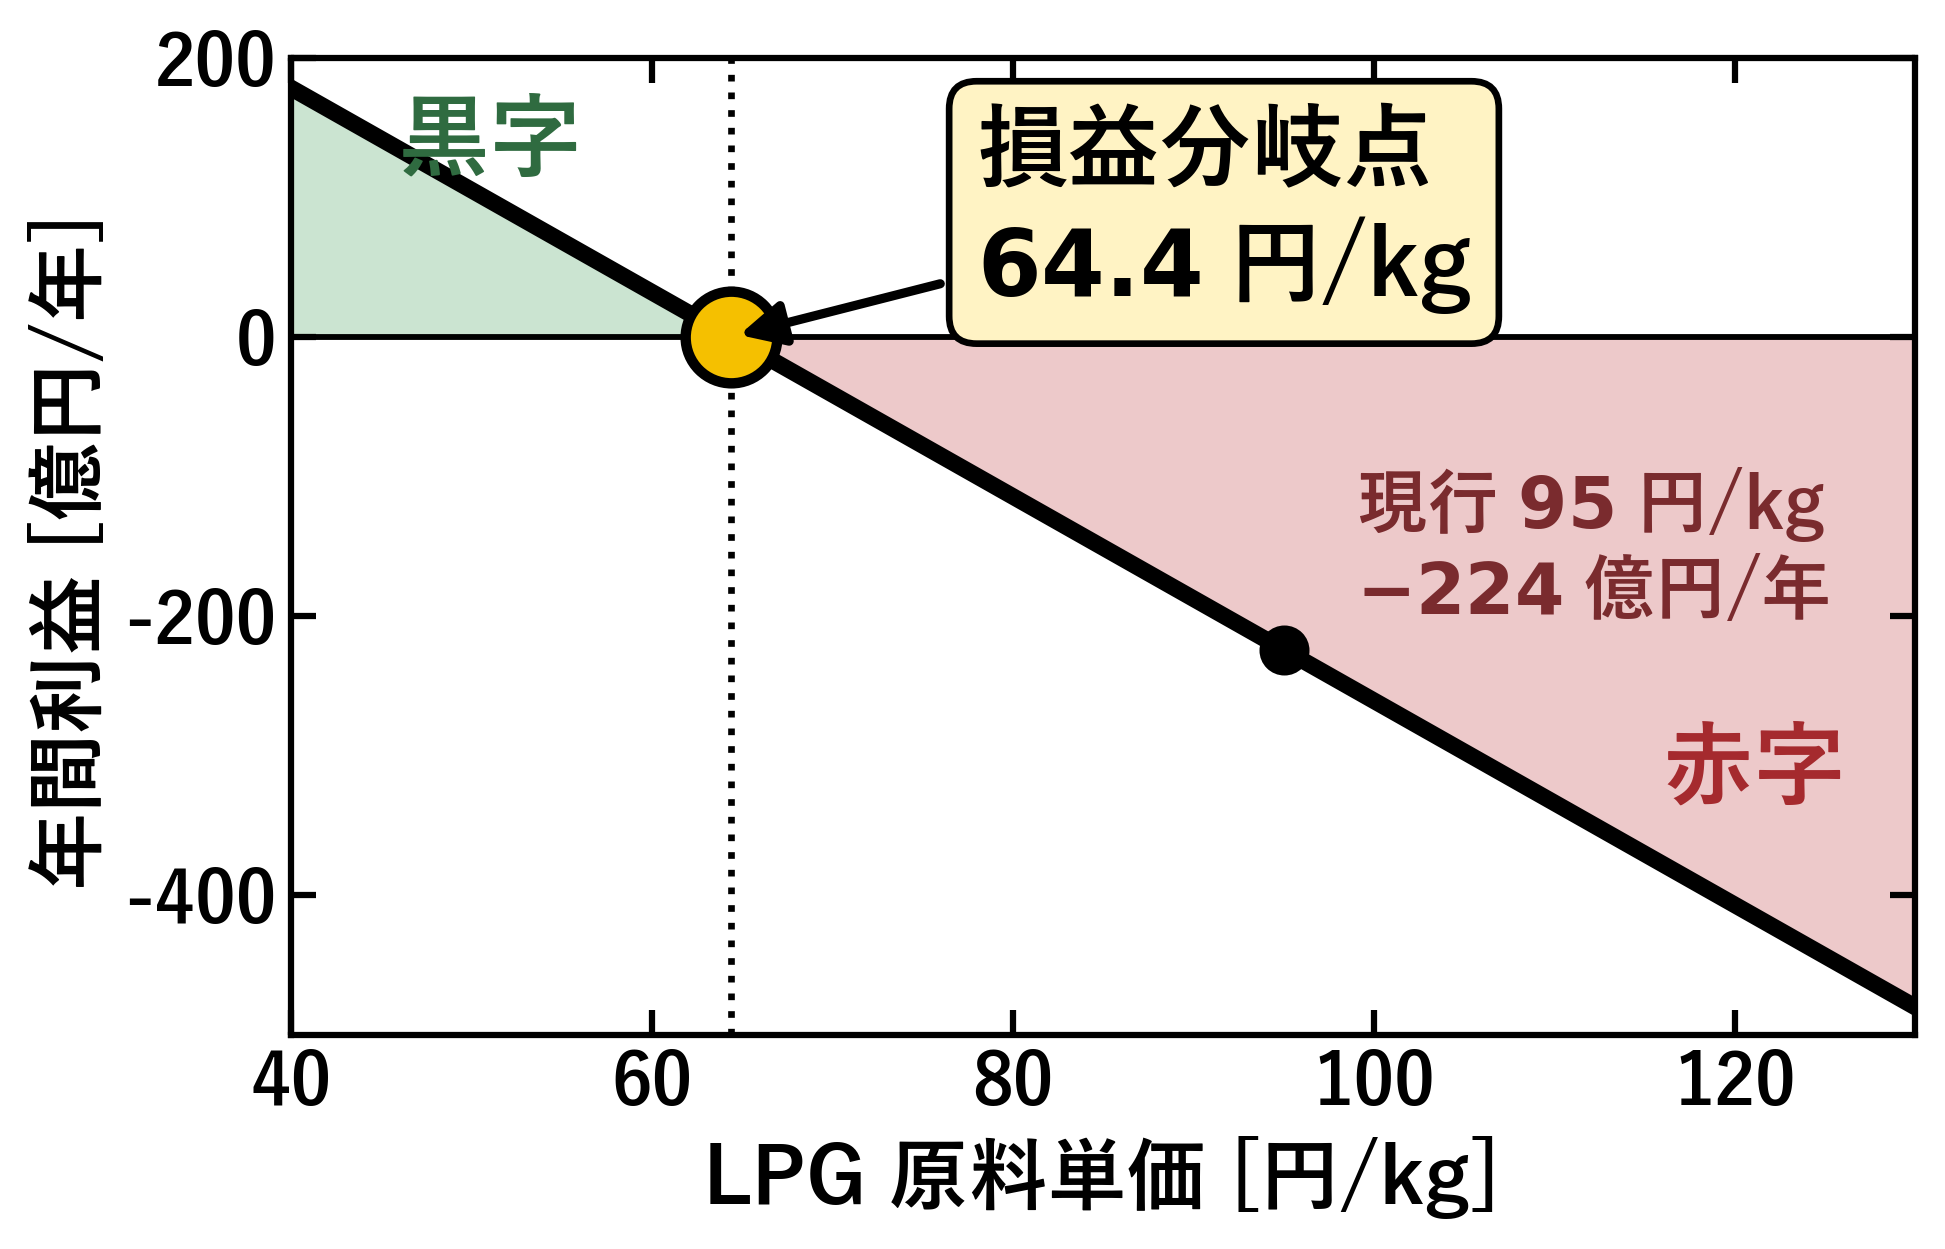
\includegraphics[width=\linewidth]{breakeven_slide}
    \end{column}
  \end{columns}

  \vspace{0.6em}

  % ===== 中段：結言（枠）=======================================
  {\setlength{\fboxsep}{6pt}\setlength{\fboxrule}{1.2pt}%
   \fcolorbox{HeaderBlue}{HiBlue!10}{%
    \begin{minipage}{\dimexpr\linewidth-16pt}
     {\footnotesize\bfseries\color{HeaderBlue} 結言}\quad
     {\small LPG から PDH でプロピレン {\boldmath$402$} kt/年・{\boldmath$99.5$} wt\% を製造する全プロセスを設計し、\textbf{全 $23$ 変数の同時最適化で TAC を最小化}した。}
    \end{minipage}}}

  \vspace{0.55em}

  % ===== 下段：改善案 8項目（小文字・行間詰め・2列）===========
  {\footnotesize\bfseries\color{HeaderBlue} 改善案}\par
  \vspace{0.2em}
  {\scriptsize\setlength{\parskip}{0.1em}
   \begin{columns}[T,onlytextwidth]
    \begin{column}{0.5\textwidth}
      \raggedright
      $\bullet$ \textbf{触媒の選定}：高選択・高活性触媒の探索\par
      $\bullet$ \textbf{触媒形状の改良}：中心にダミーを入れ実効粒径を拡大 $\to$ 圧損低減\par
      $\bullet$ \textbf{膜の経時劣化}をモデル化し現実性能で再評価\par
      $\bullet$ \textbf{熱交換器ネットワーク HEN の本格合成}\par
      $\bullet$ 熱交換網の\textbf{最小接近温度差 $\Delta T_{\min}$ を最適化変数に追加}\par
    \end{column}
    \begin{column}{0.5\textwidth}
      \raggedright
      $\bullet$ \textbf{反応速度論・選択率モデル}の高精度化\par
      $\bullet$ \textbf{非定常・動特性／制御性}の検討\par
      $\bullet$ \textbf{多目的最適化}：TAC に $\mathrm{CO_2}$・安全性を併せ評価\par
      $\bullet$ \textbf{安価 LPG の調達・立地}最適化と不確実性下のロバスト設計\par
    \end{column}
   \end{columns}}

\end{frame}

\end{document}
